% ============================================================
% Question Bank: ch04-06 Rewriting Expressions to Solve Problems
% Topic Title: Rewriting Expressions to Solve Problems
% CCSS: 7.EE.A.2
% Questions: 30 (18 MC + 7 SA + 5 Graphical)
% ============================================================

% --- Multiple Choice Questions (18) ---

\begin{practiceQuestion}{4-6-q01}{mc}
\begin{questionText}
Which expression is equivalent to $x + 0.06x$?
\end{questionText}
\choiceA{$0.06x$}
\choiceB{$1.6x$}
\choiceC{$1.06x$}
\choiceD{$6.01x$}
\correctAnswer{C}
\explanation{Factor out $x$: $x + 0.06x = (1 + 0.06)x = 1.06x$. This represents a $6\%$ increase.}
\end{practiceQuestion}

\begin{practiceQuestion}{4-6-q02}{mc}
\begin{questionText}
A store offers $20\%$ off. Which expression gives the sale price of an item that normally costs $p$ dollars?
\end{questionText}
\choiceA{$p - 20$}
\choiceB{$0.20p$}
\choiceC{$0.80p$}
\choiceD{$1.20p$}
\correctAnswer{C}
\explanation{A $20\%$ discount means you keep $80\%$: $p - 0.20p = 0.80p$.}
\end{practiceQuestion}

\begin{practiceQuestion}{4-6-q03}{mc}
\begin{questionText}
Rewrite $a + 0.15a$ as a single term. What does the result tell you?
\end{questionText}
\choiceA{$1.15a$ — a $15\%$ increase over $a$}
\choiceB{$0.15a$ — $15\%$ of $a$}
\choiceC{$15a$ — $15$ times $a$}
\choiceD{$1.15a$ — $a$ decreased by $15\%$}
\correctAnswer{A}
\explanation{$a + 0.15a = 1.15a$. This means the total is $115\%$ of the original, which is a $15\%$ increase.}
\end{practiceQuestion}

\begin{practiceQuestion}{4-6-q04}{mc}
\begin{questionText}
Which two expressions are equivalent?
\end{questionText}
\choiceA{$n - 0.25n$ and $0.25n$}
\choiceB{$n - 0.25n$ and $0.75n$}
\choiceC{$n + 0.25n$ and $0.75n$}
\choiceD{$n - 0.25n$ and $1.25n$}
\correctAnswer{B}
\explanation{$n - 0.25n = (1 - 0.25)n = 0.75n$. A $25\%$ decrease means keeping $75\%$.}
\end{practiceQuestion}

\begin{practiceQuestion}{4-6-q05}{mc}
\begin{questionText}
Simplify $3(x + 5) - 2x$.
\end{questionText}
\choiceA{$x + 15$}
\choiceB{$x + 5$}
\choiceC{$5x + 15$}
\choiceD{$x - 15$}
\correctAnswer{A}
\explanation{Expand: $3x + 15 - 2x$. Combine: $(3x - 2x) + 15 = x + 15$.}
\end{practiceQuestion}

\begin{practiceQuestion}{4-6-q06}{mc}
\begin{questionText}
A shirt costs $\$s$. Sales tax is $8\%$. Which expression gives the total cost?
\end{questionText}
\choiceA{$s + 8$}
\choiceB{$s + 0.8s$}
\choiceC{$1.08s$}
\choiceD{$0.08s$}
\correctAnswer{C}
\explanation{Tax is $0.08s$. Total: $s + 0.08s = 1.08s$.}
\end{practiceQuestion}

\begin{practiceQuestion}{4-6-q07}{mc}
\begin{questionText}
Rewrite $c - 0.10c$ as a single term.
\end{questionText}
\choiceA{$0.10c$}
\choiceB{$-0.10c$}
\choiceC{$0.90c$}
\choiceD{$1.10c$}
\correctAnswer{C}
\explanation{$c - 0.10c = (1 - 0.10)c = 0.90c$. This represents a $10\%$ decrease.}
\end{practiceQuestion}

\begin{practiceQuestion}{4-6-q08}{mc}
\begin{questionText}
A worker earns $\$w$ per hour. After a $5\%$ raise, which expression gives the new hourly wage?
\end{questionText}
\choiceA{$w + 5$}
\choiceB{$w + 0.5w$}
\choiceC{$1.05w$}
\choiceD{$0.95w$}
\correctAnswer{C}
\explanation{A $5\%$ raise means $w + 0.05w = 1.05w$.}
\end{practiceQuestion}

\begin{practiceQuestion}{4-6-q09}{mc}
\begin{questionText}
Which expression is a simplified form of $4(2n + 3) - 3(n - 1)$?
\end{questionText}
\choiceA{$5n + 15$}
\choiceB{$5n + 9$}
\choiceC{$11n + 15$}
\choiceD{$5n + 11$}
\correctAnswer{A}
\explanation{Expand: $8n + 12 - 3n + 3$. Combine: $(8n - 3n) + (12 + 3) = 5n + 15$.}
\end{practiceQuestion}

\begin{practiceQuestion}{4-6-q10}{mc}
\begin{questionText}
A coupon takes $\$5$ off, then you pay $7\%$ tax on the reduced price. If the original price is $p$, which expression gives the final cost?
\end{questionText}
\choiceA{$1.07(p - 5)$}
\choiceB{$1.07p - 5$}
\choiceC{$0.93p - 5$}
\choiceD{$(p - 5) + 0.07p$}
\correctAnswer{A}
\explanation{First discount: $p - 5$. Then add $7\%$ tax to the reduced price: $1.07(p - 5)$.}
\end{practiceQuestion}

\begin{practiceQuestion}{4-6-q11}{mc}
\begin{questionText}
A population increases by $3\%$ each year. If the current population is $P$, which expression gives the population after one year?
\end{questionText}
\choiceA{$P + 3$}
\choiceB{$0.03P$}
\choiceC{$1.03P$}
\choiceD{$0.97P$}
\correctAnswer{C}
\explanation{A $3\%$ increase means $P + 0.03P = 1.03P$.}
\end{practiceQuestion}

\begin{practiceQuestion}{4-6-q12}{mc}
\begin{questionText}
Which is equivalent to ``increase $x$ by $30\%$, then decrease the result by $30\%$''?
\end{questionText}
\choiceA{$x$}
\choiceB{$0.91x$}
\choiceC{$1.00x$}
\choiceD{$0.70x$}
\correctAnswer{B}
\explanation{Increase by $30\%$: $1.30x$. Decrease by $30\%$: $0.70 \times 1.30x = 0.91x$. The result is NOT the original.}
\end{practiceQuestion}

\begin{practiceQuestion}{4-6-q13}{mc}
\begin{questionText}
Rewrite $5(a - 2) + 3a$ in simplest form.
\end{questionText}
\choiceA{$8a - 10$}
\choiceB{$8a - 2$}
\choiceC{$2a - 10$}
\choiceD{$8a + 10$}
\correctAnswer{A}
\explanation{Expand: $5a - 10 + 3a$. Combine: $8a - 10$.}
\end{practiceQuestion}

\begin{practiceQuestion}{4-6-q14}{mc}
\begin{questionText}
A movie ticket costs $\$t$. Three friends buy tickets and split a $\$6$ popcorn equally. Which expression gives each person's total cost?
\end{questionText}
\choiceA{$3t + 6$}
\choiceB{$t + 6$}
\choiceC{$t + 2$}
\choiceD{$\frac{t + 6}{3}$}
\correctAnswer{C}
\explanation{Each person pays $t$ for a ticket plus $\frac{6}{3} = 2$ for popcorn. Total per person: $t + 2$.}
\end{practiceQuestion}

\begin{practiceQuestion}{4-6-q15}{mc}
\begin{questionText}
Which pair shows $p - 0.35p$ rewritten?
\end{questionText}
\choiceA{$0.35p$}
\choiceB{$0.65p$}
\choiceC{$1.35p$}
\choiceD{$-0.35p$}
\correctAnswer{B}
\explanation{$p - 0.35p = (1 - 0.35)p = 0.65p$. This means keeping $65\%$ of the original.}
\end{practiceQuestion}

\begin{practiceQuestion}{4-6-q16}{mc}
\begin{questionText}
A rectangle has width $w$ and length $3w + 2$. The perimeter is $2w + 2(3w + 2)$. Which is the simplified form?
\end{questionText}
\choiceA{$8w + 4$}
\choiceB{$6w + 4$}
\choiceC{$8w + 2$}
\choiceD{$5w + 4$}
\correctAnswer{A}
\explanation{$2w + 2(3w + 2) = 2w + 6w + 4 = 8w + 4$.}
\end{practiceQuestion}

\begin{practiceQuestion}{4-6-q17}{mc}
\begin{questionText}
``Buy 3, get 1 free'' on items costing $\$d$ each. What is the price per item if you buy 4?
\end{questionText}
\choiceA{$d$}
\choiceB{$\frac{3d}{4}$}
\choiceC{$\frac{d}{4}$}
\choiceD{$\frac{4d}{3}$}
\correctAnswer{B}
\explanation{You pay for $3$ items ($3d$) but get $4$. Price per item: $\frac{3d}{4} = 0.75d$, a $25\%$ discount per item.}
\end{practiceQuestion}

\begin{practiceQuestion}{4-6-q18}{mc}
\begin{questionText}
Which shows that $2(x + 4) + 3(x + 4)$ can be rewritten using factoring?
\end{questionText}
\choiceA{$5(x + 4)$}
\choiceB{$6(x + 4)$}
\choiceC{$5x + 20$}
\choiceD{Both A and C}
\correctAnswer{D}
\explanation{$2(x + 4) + 3(x + 4) = (2 + 3)(x + 4) = 5(x + 4) = 5x + 20$. Both the factored and expanded forms are correct equivalent expressions.}
\end{practiceQuestion}

% --- Short Answer Questions (7) ---

\begin{practiceQuestion}{4-6-q19}{sa}
\begin{questionText}
Rewrite $m + 0.12m$ as a single term and explain what it represents.
\end{questionText}
\correctAnswer{$1.12m$; a $12\%$ increase}
\explanation{$m + 0.12m = (1 + 0.12)m = 1.12m$. This means the total is $112\%$ of the original — a $12\%$ increase.}
\end{practiceQuestion}

\begin{practiceQuestion}{4-6-q20}{sa}
\begin{questionText}
A bike costs $\$b$. It is on sale for $15\%$ off. Write two equivalent expressions for the sale price.
\end{questionText}
\correctAnswer{$b - 0.15b$ and $0.85b$}
\explanation{The discount is $0.15b$. Sale price: $b - 0.15b$. Factor: $(1 - 0.15)b = 0.85b$.}
\end{practiceQuestion}

\begin{practiceQuestion}{4-6-q21}{sa}
\begin{questionText}
Simplify $2(3x + 5) - (4x - 3)$ and write in simplest form.
\end{questionText}
\correctAnswer{$2x + 13$}
\explanation{Expand: $6x + 10 - 4x + 3$. Combine: $(6x - 4x) + (10 + 3) = 2x + 13$.}
\end{practiceQuestion}

\begin{practiceQuestion}{4-6-q22}{sa}
\begin{questionText}
Show that ``increase by $50\%$ and then decrease by $50\%$'' does NOT give back the original price. Use a starting price of $\$80$.
\end{questionText}
\correctAnswer{$\$60$, not $\$80$}
\explanation{Increase $\$80$ by $50\%$: $80 \times 1.50 = \$120$. Decrease $\$120$ by $50\%$: $120 \times 0.50 = \$60$. The result is $\$60$, not the original $\$80$.}
\end{practiceQuestion}

\begin{practiceQuestion}{4-6-q23}{sa}
\begin{questionText}
A gym has a $\$25$ monthly fee and charges $\$3$ per class. Another gym charges $\$5$ per class with no monthly fee. Write expressions for each, and find when they cost the same for $c$ classes.
\end{questionText}
\correctAnswer{Gym 1: $3c + 25$; Gym 2: $5c$; same when $c = 12.5$, so about $12$--$13$ classes}
\explanation{Set equal: $3c + 25 = 5c$. Solve: $25 = 2c$, so $c = 12.5$. At $12$ or fewer classes, Gym 2 is cheaper. At $13$ or more, Gym 1 is cheaper.}
\end{practiceQuestion}

\begin{practiceQuestion}{4-6-q24}{sa}
\begin{questionText}
Rewrite $6(x + 2) - 3(x + 2)$ in two ways: factored form and expanded form.
\end{questionText}
\correctAnswer{Factored: $3(x + 2)$; Expanded: $3x + 6$}
\explanation{Factor: $(6 - 3)(x + 2) = 3(x + 2)$. Expand: $3x + 6$.}
\end{practiceQuestion}

\begin{practiceQuestion}{4-6-q25}{sa}
\begin{questionText}
An item costs $\$d$. After a $40\%$ markup and then a $25\%$ discount, what is the final price? Is this higher or lower than the original?
\end{questionText}
\correctAnswer{$1.05d$; higher by $5\%$}
\explanation{Markup: $1.40d$. Discount: $0.75 \times 1.40d = 1.05d$. The final price is $5\%$ more than the original.}
\end{practiceQuestion}

% --- Graphical Questions (3 GMC + 2 GSA) ---

\begin{practiceQuestion}{4-6-q26}{gmc}
\begin{questionText}
The diagram below shows the original price and the sale price of an item. Which expression represents the sale price?

\begin{center}
\begin{tikzpicture}[scale=0.7]
  % Original price bar
  \node[left, font=\bfseries] at (0,2.5) {Original:};
  \fill[funBlue!30] (1,2) rectangle (9,3);
  \draw[thick] (1,2) rectangle (9,3);
  \node at (5,2.5) {$p$};
  % Sale price bar (75% of original)
  \node[left, font=\bfseries] at (0,0.5) {Sale:};
  \fill[funGreen!30] (1,0) rectangle (7,1);
  \draw[thick] (1,0) rectangle (7,1);
  \node at (4,0.5) {?};
  % Discount portion
  \fill[funRed!20] (7,0) rectangle (9,1);
  \draw[thick, dashed] (7,0) rectangle (9,1);
  \node at (8,0.5) {\small$25\%$};
\end{tikzpicture}
\end{center}
\end{questionText}
\choiceA{$0.25p$}
\choiceB{$p - 25$}
\choiceC{$1.25p$}
\choiceD{$0.75p$}
\correctAnswer{D}
\explanation{The diagram shows $25\%$ is removed. The sale price is $p - 0.25p = 0.75p$, or $75\%$ of the original.}
\end{practiceQuestion}

\begin{practiceQuestion}{4-6-q27}{gmc}
\begin{questionText}
The table shows a price with different adjustments. Which row shows an equivalent rewritten expression?

\begin{center}
\begin{tabular}{|c|c|c|}
\hline
\textbf{Row} & \textbf{Original Form} & \textbf{Rewritten Form} \\
\hline
1 & $d + 0.07d$ & $1.07d$ \\
\hline
2 & $d - 0.30d$ & $1.30d$ \\
\hline
3 & $d + 0.50d$ & $0.50d$ \\
\hline
4 & $d - 0.15d$ & $1.15d$ \\
\hline
\end{tabular}
\end{center}
\end{questionText}
\choiceA{Row 1}
\choiceB{Row 2}
\choiceC{Row 3}
\choiceD{Row 4}
\correctAnswer{A}
\explanation{Row 1: $d + 0.07d = (1 + 0.07)d = 1.07d$ \checkmark. Row 2 should be $0.70d$. Row 3 should be $1.50d$. Row 4 should be $0.85d$.}
\end{practiceQuestion}

\begin{practiceQuestion}{4-6-q28}{gmc}
\begin{questionText}
The two models below show different ways to compute the cost of $5$ notebooks at $\$n$ each with $10\%$ sales tax. Which model is correct?

\begin{center}
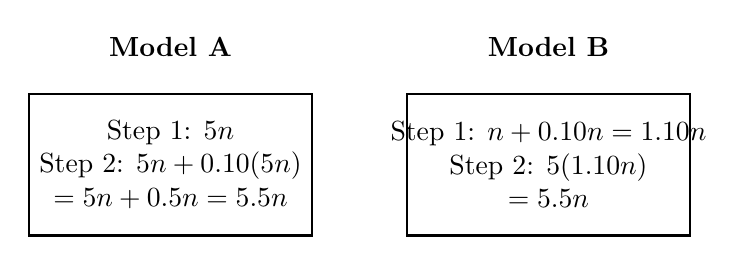
\begin{tikzpicture}[scale=0.6]
  % Model A
  \node[font=\bfseries] at (3,4) {Model A};
  \draw[thick] (0,0) rectangle (6,3);
  \node[align=center] at (3,1.5) {Step 1: $5n$\\Step 2: $5n + 0.10(5n)$\\$= 5n + 0.5n = 5.5n$};

  % Model B
  \begin{scope}[xshift=8cm]
  \node[font=\bfseries] at (3,4) {Model B};
  \draw[thick] (0,0) rectangle (6,3);
  \node[align=center] at (3,1.5) {Step 1: $n + 0.10n = 1.10n$\\Step 2: $5(1.10n)$\\$= 5.5n$};
  \end{scope}
\end{tikzpicture}
\end{center}
\end{questionText}
\choiceA{Only Model A is correct}
\choiceB{Only Model B is correct}
\choiceC{Both models are correct}
\choiceD{Neither model is correct}
\correctAnswer{C}
\explanation{Both give $5.5n$. Model A taxes the total; Model B taxes each item first. Both are equivalent because $5(1.10n) = 5.5n = 5n + 0.5n$.}
\end{practiceQuestion}

\begin{practiceQuestion}{4-6-q29}{gsa}
\begin{questionText}
A phone plan has the pricing shown. Write two equivalent expressions for the total monthly cost if you use $d$ GB of data.

\begin{center}
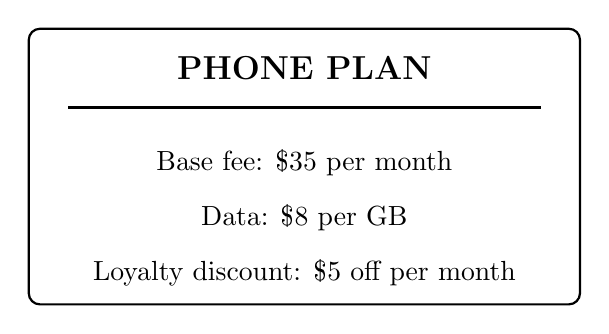
\begin{tikzpicture}
  \draw[thick, rounded corners] (0,0) rectangle (7,3.5);
  \node[font=\bfseries\large] at (3.5,3) {PHONE PLAN};
  \draw[thick] (0.5,2.5) -- (6.5,2.5);
  \node[align=left] at (3.5,1.8) {Base fee: \$35 per month};
  \node[align=left] at (3.5,1.1) {Data: \$8 per GB};
  \node[align=left] at (3.5,0.4) {Loyalty discount: \$5 off per month};
\end{tikzpicture}
\end{center}
\end{questionText}
\correctAnswer{$35 + 8d - 5 = 8d + 30$}
\explanation{Base fee plus data minus discount: $35 + 8d - 5$. Combine constants: $8d + 30$. Both forms are equivalent.}
\end{practiceQuestion}

\begin{practiceQuestion}{4-6-q30}{gsa}
\begin{questionText}
The diagram shows the price changes for a jacket. What is the final price? Express your answer as a single term in terms of the original price $p$.

\begin{center}
\begin{tikzpicture}[scale=0.7]
  % Step boxes
  \node[draw, thick, rounded corners, fill=funBlue!15, minimum width=3cm, minimum height=1.2cm] (A) at (0,0) {Original: $p$};
  \draw[->, ultra thick] (1.8,0) -- (3.2,0);
  \node[draw, thick, rounded corners, fill=funOrange!15, minimum width=3cm, minimum height=1.2cm] (B) at (5.5,0) {\small Markup $20\%$};
  \draw[->, ultra thick] (7.3,0) -- (8.7,0);
  \node[draw, thick, rounded corners, fill=funGreen!15, minimum width=3cm, minimum height=1.2cm] (C) at (11,0) {\small Discount $10\%$};
  \draw[->, ultra thick] (12.8,0) -- (14.2,0);
  \node[draw, thick, rounded corners, fill=funRed!15, minimum width=3cm, minimum height=1.2cm] (D) at (16.5,0) {Final: ?};
\end{tikzpicture}
\end{center}
\end{questionText}
\correctAnswer{$1.08p$}
\explanation{Markup $20\%$: $1.20p$. Discount $10\%$: $0.90 \times 1.20p = 1.08p$. The final price is $108\%$ of the original, which is an $8\%$ net increase.}
\end{practiceQuestion}
